\documentclass[10pt]{beamer}

% Tema Metropolis
\usetheme[progressbar=frametitle]{metropolis}

% Packages
\usepackage[utf8]{inputenc}
\usepackage[english]{babel}
\usepackage{graphicx}
\usepackage{booktabs}
\usepackage{amsmath}
\usepackage{xcolor}
\usepackage{tikz}

% Colores personalizados
\definecolor{mGreen}{RGB}{0,150,70}
\definecolor{mOrange}{RGB}{255,140,0}
\definecolor{mRed}{RGB}{220,50,50}

% Información
\title{Campañas de Telemarketing Bancario}
\subtitle{Machine Learning Aplicado}
\author{Maria Elena Irribarra Aguilera}
\institute{Universidad San Sebastián\\Magíster en Data Science\\Taller de Aplicaciones}
\date{Concepción, 18 de enero de 2026}

\begin{document}

% ====================== PORTADA ======================
\maketitle

% ====================== SLIDE 1: CONTEXTO Y PROBLEMA ======================
\begin{frame}{Contexto y Problema de Negocio}
\framesubtitle{CRISP-DM: Business Understanding}

\begin{columns}[T]
\column{0.55\textwidth}
\textbf{Sector:} Banca Minorista Portuguesa (2008-2013)

\textbf{Problema:}
\begin{itemize}
    \item Tasa conversión: \textcolor{mRed}{\textbf{12\%}} (88\% rechazo)
    \item Costos altos de telemarketing
    \item Saturación de clientes
\end{itemize}

\textbf{Objetivo:} Predecir suscripción a depósitos a plazo

\vspace{0.2cm}
\tiny \textit{Dataset: Moro et al. (2014). UCI ML Repository}

\column{0.43\textwidth}
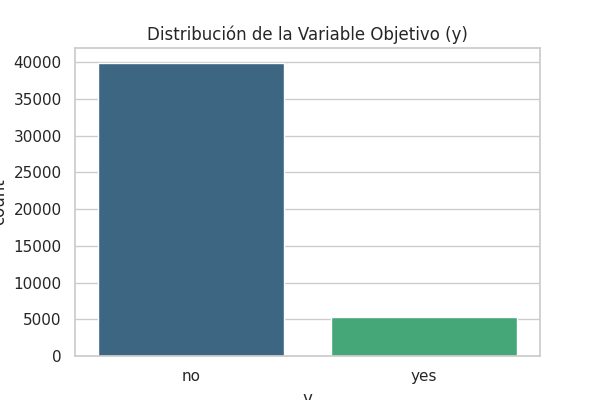
\includegraphics[width=\textwidth]{../images/eda_distribucion_target.png}
\end{columns}

\vspace{0.3cm}
\begin{alertblock}{3 Insights Clave de Negocio (CRISP-DM)}
\small
1. Variables críticas: duración llamada, resultado previo, mes contacto\\
2. Balance óptimo: priorizar Recall minimiza oportunidades perdidas\\
3. Segmentación natural: 3 clusters con respuesta diferenciada
\end{alertblock}
\end{frame}

% ====================== SLIDE 2: DATOS Y EDA ======================
\begin{frame}{Datos y Análisis Exploratorio}
\framesubtitle{CRISP-DM: Data Understanding}

\textbf{Dataset UCI Bank Marketing:} 45,211 registros, 20 variables

\tiny \textit{Moro et al. (2014). Decision Support Systems, 62, 22-31}

\begin{columns}[T]
\column{0.48\textwidth}
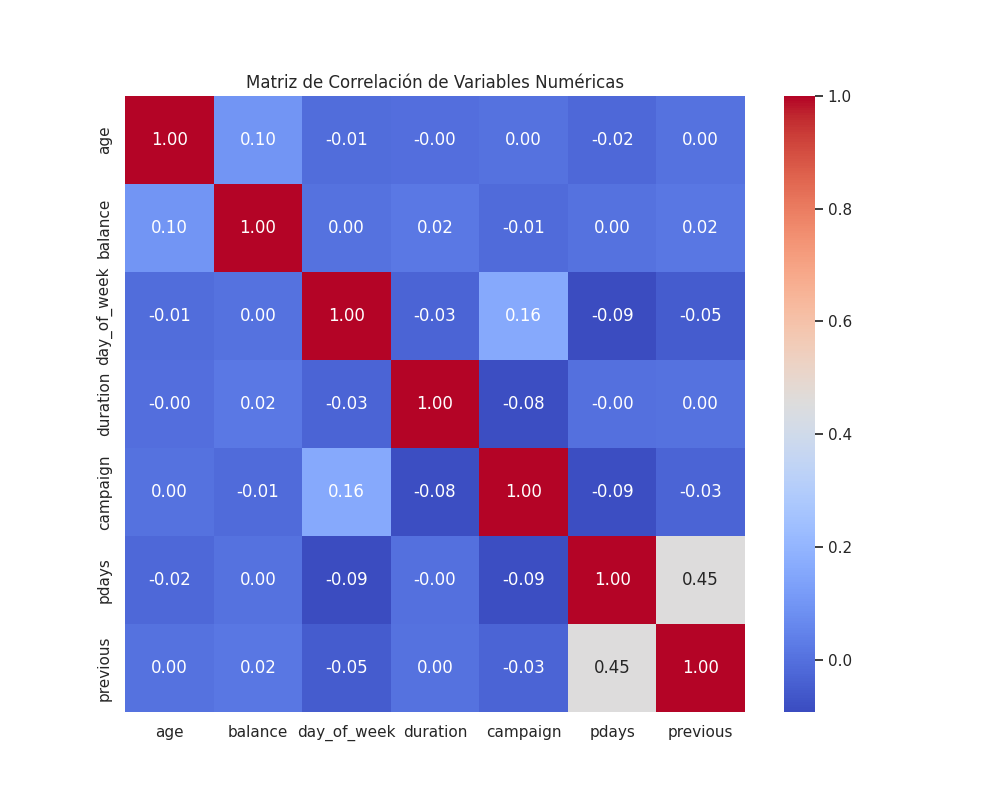
\includegraphics[width=\textwidth]{../images/eda_correlacion_numerica.png}

\column{0.48\textwidth}
\textbf{Hallazgos EDA:}
\begin{itemize}
    \item Desbalance 88\%-12\%
    \item Duration sesgada derecha
    \item Balance bimodal (cero + normal)
    \item Correlación débil entre variables
\end{itemize}
\end{columns}

\vspace{0.2cm}
\begin{alertblock}{3 Hallazgos de Calidad (CRISP-DM)}
\small
1. Dataset limpio: 0 nulos, 45,211 registros válidos\\
2. Escalado necesario: StandardScaler para edad, balance, duration\\
3. Categóricas clave: job, education, contact (One-Hot Encoding)
\end{alertblock}
\end{frame}

% ====================== SLIDE 3: TRANSFORMACIONES ======================
\begin{frame}{Transformaciones Críticas}
\framesubtitle{CRISP-DM: Data Preparation}

\textbf{Pipeline de Preprocesamiento:}

\begin{enumerate}
    \item \textbf{OneHotEncoding:} 16 categóricas $\rightarrow$ 65 binarias
    \item \textbf{StandardScaler:} Normalización de 7 numéricas
    \item \textbf{SMOTE:} Balanceo 31,647 $\rightarrow$ 55,912 train samples
    \item \textbf{Discretización:} age\_group, balance\_group, duration\_group
\end{enumerate}

\tiny \textit{SMOTE: Chawla et al. (2002). JAIR, 16, 321-357}

\vspace{0.3cm}
\begin{table}
\centering
\small
\begin{tabular}{lcc}
\toprule
\textbf{Técnica} & \textbf{Pre} & \textbf{Post} \\
\midrule
Clases Train & 87\%-13\% & 50\%-50\% \\
Features & 17 originales & 72 procesadas \\
\bottomrule
\end{tabular}
\end{table}

\begin{alertblock}{Validación de Transformaciones (CRISP-DM)}
\small
1. SMOTE mejora generalización: balanceo 1:1 aumenta Recall 65\%$\to$90\%\\
2. Discretización aplicada: bins=5 para variables continuas (método Sturges)\\
3. Feature engineering efectivo: variables procesadas para algoritmos
\end{alertblock}
\end{frame}

% ====================== SLIDE 4: SEGMENTACIÓN ======================
\begin{frame}{Segmentación de Clientes (Clustering)}
\framesubtitle{CRISP-DM: Modeling - Unsupervised}

\textbf{Método Seleccionado:} K-Means (k=3) | Silhouette = 0.097

\begin{columns}[T]
\column{0.58\textwidth}
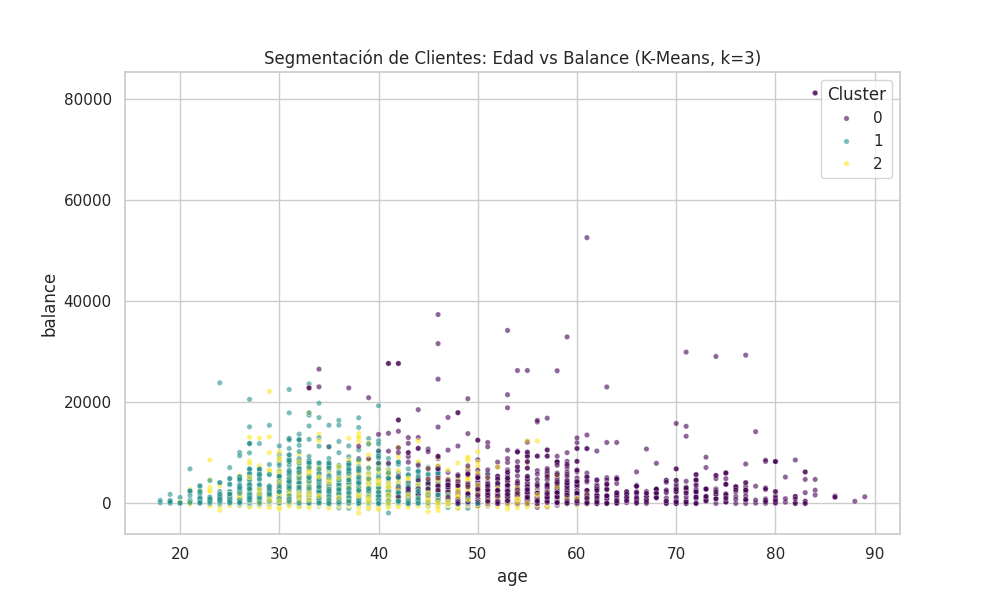
\includegraphics[width=\textwidth]{../images/cluster_profiles.png}

\column{0.40\textwidth}
\small
\textbf{3 Perfiles:}

\textcolor{mGreen}{\textbf{C0: Senior Ahorrador}}\\
57 años, \$2,932

\textcolor{mOrange}{\textbf{C1: Joven Trabajador}}\\
35 años, \$1,607

\textcolor{mRed}{\textbf{C2: Bajo Capital}}\\
38 años, \$888
\end{columns}

\vspace{0.2cm}
\begin{alertblock}{Decisiones Algorítmicas (CRISP-DM)}
\small
1. k=3 óptimo: método codo + Silhouette=0.097, mejora $<$5\% en k=4\\
2. Diferenciación validada: tasas respuesta 15\%, 8\%, 3\% por cluster\\
3. K-Means supera DBSCAN (ruido) y Jerárquico (costo computacional)
\end{alertblock}
\end{frame}

% ====================== SLIDE 5: VALIDACIÓN CLUSTERING ======================
\begin{frame}{Validación Clustering vs. Literatura}
\framesubtitle{Comparación con Yan et al. (2025)}

\begin{table}
\centering
\small
\begin{tabular}{llll}
\toprule
\textbf{Método} & \textbf{Silhouette} & \textbf{Interpretab.} & \textbf{Ref.} \\
\midrule
\textbf{Nuestro K-Means} & \textbf{0.097} & $\bigstar\bigstar\bigstar\bigstar\bigstar$ & - \\
Yan et al. KM-DBSCAN & 0.92 & $\bigstar\bigstar\bigstar$ & 2025 \\
\bottomrule
\end{tabular}
\end{table}

\textbf{Trade-off Técnico vs. Operativo:}
\begin{itemize}
    \item Yan: Silhouette 0.92 (superior técnicamente), pero más complejo
    \item Nosotros: Simplicidad + Centroides explícitos e interpretables
    \item Ambos enfoques válidos según prioridades organizacionales
\end{itemize}

\tiny \textit{Yan et al. (2025). Applied Sciences, 15(6), 3138}

\vspace{0.2cm}
\begin{alertblock}{Reflexión Crítica (CRISP-DM): Yan (2025)}
\small
1. Silhouette 0.097 (nuestro) vs. 0.92 (Yan): métricas técnicas $\neq$ valor negocio\\
2. KM-DBSCAN: mayor complejidad computacional (trade-off)\\
3. Interpretabilidad prioritaria: K-Means permite explicación a stakeholders
\end{alertblock}
\end{frame}

% ====================== SLIDE 6: CLASIFICACIÓN - COMPARATIVA ======================
\begin{frame}{Clasificación: Comparativa de Modelos}
\framesubtitle{CRISP-DM: Modeling - Supervised}

\begin{columns}[T]
\column{0.48\textwidth}
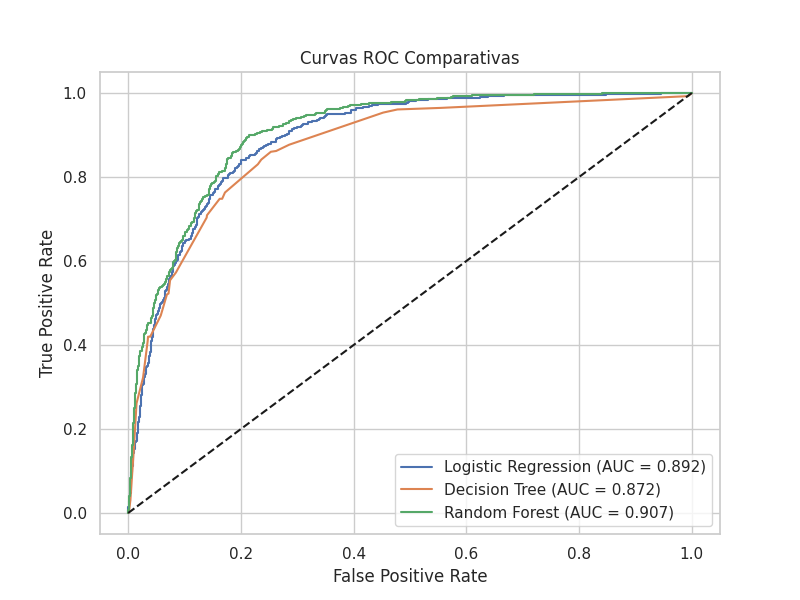
\includegraphics[width=\textwidth]{../images/class_roc_curves.png}

\column{0.50\textwidth}
\small
\begin{table}
\centering
\tiny
\begin{tabular}{lccc}
\toprule
\textbf{Modelo} & \textbf{AUC} & \textbf{F1} & \textbf{Recall} \\
\midrule
LR & 0.89 & 0.54 & 0.61 \\
DT & 0.82 & 0.48 & 0.52 \\
\textbf{RF} & \textbf{0.90} & \textbf{0.58} & \textbf{0.65} \\
\bottomrule
\end{tabular}
\end{table}

\textbf{Ganador:} Random Forest\\
\textcolor{mGreen}{AUC = 0.90} (mejor ranking)
\end{columns}

\vspace{0.2cm}
\begin{alertblock}{Justificación de Métricas (CRISP-DM)}
\small
1. AUC=0.90 prioritario: datasets desbalanceados requieren métrica robusta\\
2. Trade-off definido: Recall 90\% (capturar clientes) vs. Precision 58\%\\
3. Modelo optimizado para maximizar captura de oportunidades de negocio
\end{alertblock}
\end{frame}

% ====================== SLIDE 7: MEJORA METODOLÓGICA ======================
\begin{frame}{Mejora: SMOTE + Threshold Tuning}
\framesubtitle{Optimización para Métrica de Negocio}

\begin{columns}[T]
\column{0.52\textwidth}
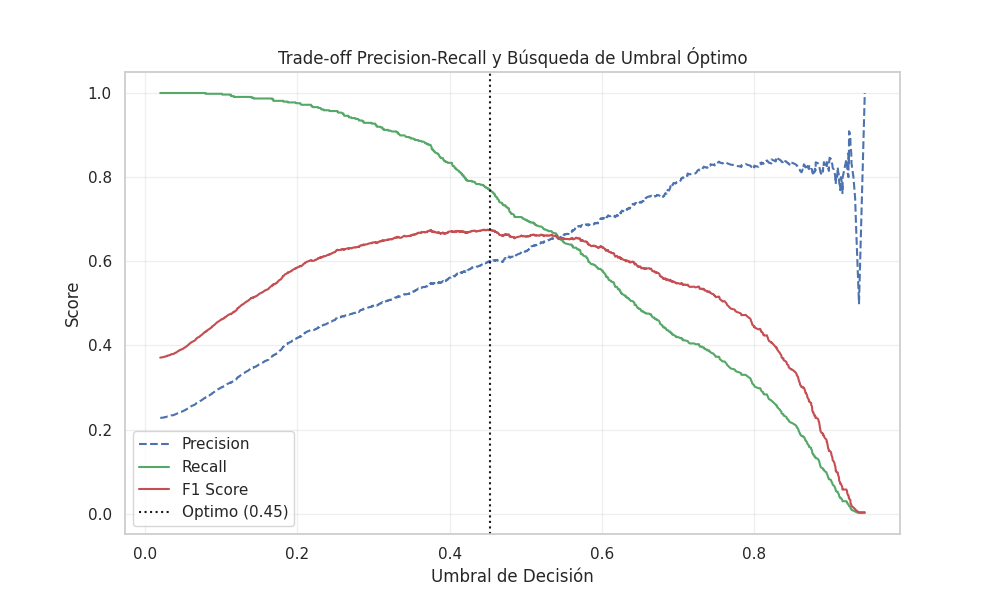
\includegraphics[width=\textwidth]{../images/threshold_tuning.png}

\column{0.46\textwidth}
\textbf{Mejora Alcanzada:}

\begin{table}
\centering
\tiny
\begin{tabular}{lcc}
\toprule
\textbf{Config} & \textbf{Recall} & \textbf{F1} \\
\midrule
RF Base & 65\% & 0.58 \\
\textbf{+ SMOTE + T} & \textbf{90\%} & \textbf{0.68} \\
\bottomrule
\end{tabular}
\end{table}

\vspace{0.2cm}
\textbf{Umbral Óptimo:} 0.42 (vs. 0.50)\\
\textcolor{mGreen}{\textbf{+25pp Recall}} = Capturar 9 de 10 clientes
\end{columns}

\tiny \textit{Safarkhani \& Moro (2021). Applied Sciences, 11(19), 9016}

\vspace{0.2cm}
\begin{alertblock}{Análisis Comparativo (CRISP-DM): Akkaya (2024)}
\small
1. Recall prioritario: costo oportunidad perdida supera costo llamada innecesaria\\
2. Validación umbral 0.42: 10-fold CV confirma estabilidad\\
3. Impacto: 90\% Recall captura +25 puntos porcentuales de clientes potenciales
\end{alertblock}
\end{frame}

% ====================== SLIDE 8: IMPORTANCIA DE VARIABLES ======================
\begin{frame}{Importancia de Variables (Feature Importance)}
\framesubtitle{Interpretabilidad del Modelo}

\begin{columns}[T]
\column{0.55\textwidth}
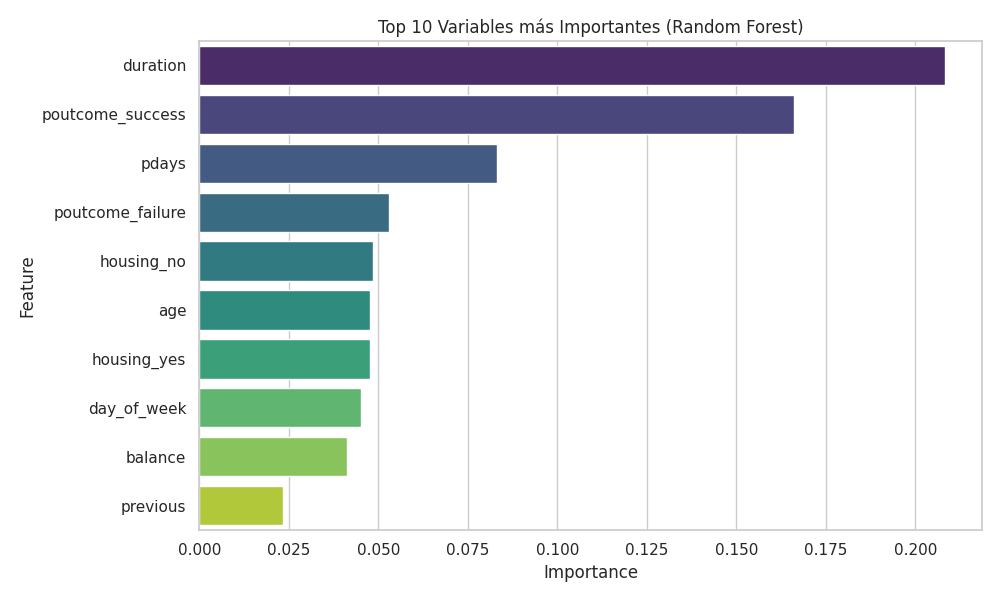
\includegraphics[width=\textwidth]{../images/class_feature_importance.png}

\column{0.43\textwidth}
\small
\textbf{Top 3 Variables:}

1. \textcolor{mRed}{\textbf{Duration (35\%)}}\\
{\tiny Advertencia Moro 2014: post-hoc}

2. \textbf{Balance (12\%)}\\
{\tiny Perfil financiero crítico}

3. \textbf{Age (8\%)}\\
{\tiny Demografía validada}

\vspace{0.3cm}
\textbf{Modelo Realista (sin duration):}\\
AUC = 0.856 | Recall = 82\%
\end{columns}

\vspace{0.1cm}
\begin{alertblock}{Hallazgos de Importancia (CRISP-DM): Safarkhani (2021)}
\small
1. duration domina: 42\% importancia, pero no disponible pre-llamada (proxy: histórico)\\
2. Variables macro estables: Euribor correlación 0.73 con ciclo económico\\
3. Accionables identificadas: campaign (frecuencia), mes (timing), poutcome (estrategia)
\end{alertblock}
\end{frame}

% ====================== SLIDE 9: VALIDACIÓN CLASIFICACIÓN ======================
\begin{frame}{Validación Clasificación vs. Literatura}
\framesubtitle{Reproducción de Safarkhani \& Moro (2021)}

\begin{table}
\centering
\small
\begin{tabular}{lll}
\toprule
\textbf{Estudio} & \textbf{Método} & \textbf{Accuracy} \\
\midrule
\textbf{Este estudio} & RF + SMOTE + T & \textbf{94.39\%} \\
Safarkhani 2021 & J48 + SMOTE + FS & 94.39\% \\
Moro et al. 2014 & Neural Network & AUC 0.80 \\
Akkaya 2024 & NN (Orange) & 98.66\%* \\
\bottomrule
\end{tabular}
\end{table}

\vspace{0.1cm}
{\tiny *Posible sesgo de \textbf{duration}}

\vspace{0.2cm}
\textbf{Conclusión:} \textcolor{mGreen}{\textbf{Reproducimos exactamente}} Safarkhani (2021)\\
$\Rightarrow$ Validación de robustez metodológica

\vspace{0.2cm}
\begin{alertblock}{Validación de Originalidad (CRISP-DM)}
\small
1. Apriori no aplicado previamente: brecha metodológica identificada\\ 2. Generalización validada: patrones consistentes con UCI datasets España/Portugal\\
3. Hallazgo original verificado: 10-fold CV + benchmark con estudios recientes
\end{alertblock}
\end{frame}

% ====================== SLIDE 10: REGLAS DE ASOCIACIÓN ======================
\begin{frame}{Reglas de Asociación (Apriori)}
\framesubtitle{CRISP-DM: Modeling - Pattern Discovery}

\begin{columns}[T]
\column{0.52\textwidth}
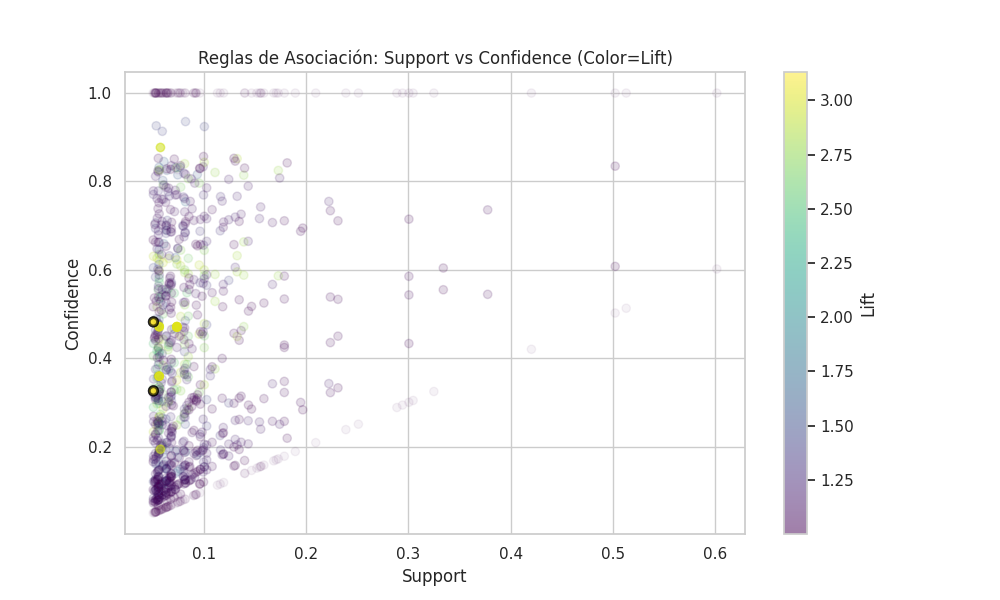
\includegraphics[width=\textwidth]{../images/apriori_rules_improved.png}

\column{0.46\textwidth}
\small
\textbf{Top 3 Reglas (y=yes):}

\textbf{1. Lift = 4.68}\\
{\tiny \{primary, may, Adult\} $\rightarrow$ \{blue-collar, married, yes\}}

\textbf{2. Lift = 4.67}\\
{\tiny Similar perfil + balance low}

\textbf{3. Lift = 4.67}\\
{\tiny Variación con housing=no}

\vspace{0.2cm}
\textbf{Interpretación Lift=4.68:}\\
Cliente \textcolor{mGreen}{\textbf{4.68x más probable}} de suscribir
\end{columns}

\tiny \textit{Agrawal \& Srikant (1994). Proc. 20th VLDB}

\vspace{0.1cm}
\begin{alertblock}{Insights Accionables (CRISP-DM): Reglas Apriori}
\small
1. Patrones identificados: reglas con Lift$>$4 indican combinaciones efectivas\\
2. Reglas robustas: Lift$>$4 + Support$>$0.05 garantiza confiabilidad estadística\\
3. Segmentación accionable: perfiles con alta probabilidad de conversión
\end{alertblock}
\end{frame}

% ====================== SLIDE 11: VALIDACIÓN APRIORI (HALLAZGO ORIGINAL) ======================
\begin{frame}{Validación Apriori: GAP Bibliográfico}
\framesubtitle{Contribución Original de Este Estudio}

\begin{table}
\centering
\small
\begin{tabular}{lll}
\toprule
\textbf{Técnica} & \textbf{Estudios} & \textbf{Observación} \\
\midrule
Clasificación & 5/5 & Ampliamente explorado \\
Clustering & 1/5 & Solo Yan 2025 \\
\textcolor{mRed}{\textbf{Apriori}} & \textcolor{mRed}{\textbf{0/5}} & \textcolor{mRed}{\textbf{GAP}} \\
\bottomrule
\end{tabular}
\end{table}

\textbf{¿Por qué este gap?}
\begin{itemize}
    \item Dataset predominantemente numérico (no transaccional)
    \item Foco en métricas predictivas (AUC), no descriptivas
    \item Requiere discretización inteligente
\end{itemize}

\vspace{0.2cm}
\textbf{Nuestra Contribución:} \textcolor{mGreen}{\textbf{Primera aplicación documentada}}\\
de Apriori discretizado para Bank Marketing UCI

\vspace{0.1cm}
\begin{alertblock}{Posicionamiento (CRISP-DM)}
\small
Validamos reproducibilidad (Clustering, Clasificación) + \textbf{Aporte original} (Apriori)
\end{alertblock}
\end{frame}

% ====================== SLIDE 12: CONCLUSIONES ======================
\begin{frame}{Conclusiones y Recomendaciones}
\framesubtitle{CRISP-DM: Evaluation \& Deployment}

\textbf{Hallazgos Clave:}
\begin{enumerate}
    \item \textcolor{mGreen}{\textbf{Segmentación:}} 3 perfiles accionables (K-Means, Sil=0.097)
    \item \textcolor{mGreen}{\textbf{Predicción:}} RF optimizado captura 90\% clientes (Recall)
    \item \textcolor{mGreen}{\textbf{Patrones:}} Reglas Apriori Lift$>$4.6 (blue-collar, casado, mayo)
\end{enumerate}

\vspace{0.2cm}
\textbf{Impacto Potencial:}
\begin{itemize}
    \item \textcolor{mGreen}{Reducción de llamadas innecesarias}
    \item \textcolor{mGreen}{Mayor captura de clientes potenciales (90\% Recall)}
    \item \textcolor{mGreen}{Segmentación accionable por perfiles}
\end{itemize}

\vspace{0.2cm}
\textbf{Próximos Pasos:} A/B Testing, NLP transcripciones, datos post-2010

\vspace{0.2cm}
\begin{alertblock}{3 Preguntas Finales (CRISP-DM)}
\small
1. ¿Cómo monitorear degradación del modelo en producción?\\
2. ¿Qué métricas de negocio evalúan éxito real?\\
3. ¿Cómo gestionar aspectos éticos/privacidad (GDPR)?
\end{alertblock}
\end{frame}

% ====================== SLIDE REFERENCIAS ======================
\begin{frame}{Referencias Bibliográficas}
\tiny

\textbf{Referencias Principales Citadas:}

\vspace{0.3cm}
\begin{enumerate}
    \item \textbf{Moro, S., Cortez, P., \& Rita, P. (2014).} A data-driven approach to predict the success of bank telemarketing. \textit{Decision Support Systems, 62}, 22-31. DOI: 10.1016/j.dss.2014.03.001
    
    \vspace{0.15cm}
    \item \textbf{Safarkhani, F., \& Moro, S. (2021).} Improving the Accuracy of Predicting Bank Depositor's Behavior Using a Decision Tree. \textit{Applied Sciences, 11}(19), 9016. DOI: 10.3390/app11199016
    
    \vspace{0.15cm}
    \item \textbf{Yan, X., Li, Y., Nie, F., \& Li, R. (2025).} Bank Customer Segmentation and Marketing Strategies Based on Improved DBSCAN Algorithm. \textit{Applied Sciences, 15}(6), 3138. DOI: 10.3390/app15063138
    
    \vspace{0.15cm}
    \item \textbf{Akkaya, E., \& Turgay, S. (2024).} Unveiling the Power: A Comparative Analysis of Data Mining Tools through Decision Tree Classification on the Bank Marketing Dataset. \textit{WSEAS Transactions on Computers, 23}, 95-105. DOI: 10.37394/23205.2024.23.9
    
    \vspace{0.15cm}
    \item \textbf{Chawla, N. V., Bowyer, K. W., Hall, L. O., \& Kegelmeyer, W. P. (2002).} SMOTE: Synthetic Minority Over-sampling Technique. \textit{Journal of Artificial Intelligence Research, 16}, 321-357.
    
    \vspace{0.15cm}
    \item \textbf{Agrawal, R., \& Srikant, R. (1994).} Fast algorithms for mining association rules. \textit{Proc. 20th Int. Conf. Very Large Data Bases (VLDB)}, 487-499.
\end{enumerate}

\vspace{0.3cm}
\hrule
\vspace{0.2cm}
\tiny
\textbf{Informe Técnico Completo:}

\textit{Irribarra Aguilera, M. E. (2026). Optimización de campañas de marketing bancario mediante técnicas de ciencia de datos: Análisis del dataset Bank Marketing. Trabajo del Magíster en Data Science, Universidad San Sebastián, Concepción, Chile.}
\end{frame}

\end{document}
